\section{Discussion}  \label{sec:disc}

\subsection{Hybrid Temporal/Spatial Imputation Methods}

Hybrid methods of temporal and spatial approaches are less common in the literature.
For example, the average of the temporal approach of linear interpolation and the spatial approach of multivariate regression has been reported[8].
Strictly speaking, this approach can be thought of as an ensemble approach between the two methods rather than a fully-integrated approach which considers both temporal and spatial aspects of WSN data.

\subsection{Parameter Setting} \label{subsec:parameter}

For both MF and TF model, we observe that the parameter setting in random split must be different from that in temporal split. Basically, we need stronger regularization in temporal split.  We provide some details and explanation here. 

Let us look at two illustrating examples.
Here we ignore bias terms for simplicity.
Random split is like Equation \ref{randomSplit_matrix}.
We have more confidence in our prediction and we rely mostly on temporal correlation, so we prefer more features and weak conventional regularization.
We also see that linear interpolation can be viewed as a solution of TRMF, in which the number of features is large and no conventional regularization is applied. 
\begin{equation}
\label{randomSplit_matrix}
\begin{bmatrix}
16 & 22 & 18\\
 ? & 22 & 19\\
18 &  ?	& 22\\
19 & 24 &  ?\\
20 & 26 & 26\\
\end{bmatrix} 
= 
\begin{bmatrix}
16 & 22 & 18\\
\mathbf{17} & 22 & 19\\
18 & \mathbf{23}	& 22\\
19 & 24 & \mathbf{24}\\
20 & 26 & 26\\
\end{bmatrix} 
\times
\begin{bmatrix}
1 & 0 & 0\\
0 & 1 & 0\\
0 & 0 & 1\\
\end{bmatrix} 
\end{equation}

Temporal split is like Equation \ref{temporalSplit_matrix}.
In contrast to temporal split case, we can't use temporal correlation to infer the missing values and we have less confidence in prediction.
We can only rely on the spatial correlation, so we prefer fewer features and stronger conventioal regularization.

\begin{equation}
\label{temporalSplit_matrix}
\begin{bmatrix}
30 & 30 & 28\\
31 & 31 & 28\\
32 &  ? & 28\\
33 &  ? & 28\\
32 &  ? & 28\\
\end{bmatrix} 
= 
\begin{bmatrix}
30 & 28\\
31 & 28\\
32 & 28\\
33 & 28\\
32 & 28\\
\end{bmatrix} 
\times
\begin{bmatrix}
1 & 1 & 0\\
0 & 0 & 1\\
\end{bmatrix} 
\end{equation}
\redtext{(should be merged with TF)}
To be specific, we share the actual values of the parameters.
Firstly, the learning rate $\eta$ is $0.04$ to $0.004$, which is chosen as the largest value that still maintains stable optimization process.
Secondly, a strong temporal regularization is always preferred.
Temporal regularization times learning rate ($\gamma \times \eta$) is set to $0.2$ in all of our experiment.
The conventional regularization is $0.001$ for temporal split and $0$ for random split.
Finally, we observe that a large $K$ doesn't lead to overfitting because SGD is a natural regularization that prefers small feature values and it may lead to several non-independent features.
The number of features $K$ is $54$ in Berkeley data set and $21$ in traffic data set, although in temporal split the $K$ may be much lowered to speed up the algorithm. 

As for the TF model, the learning rate is $0.001$ to $0.0001 $. In temporal split data, it is more easier to be over-fitting. Therefore, the conventianal regularization term should be higher than temporal split. we set conventional regularization term to 0.005 for temporal split and 0.001 for random split. Also, the larger $K$ does't lead to overfitting, In the experiment, the $K$ of TF model  is $30$ in Berkeley dataset and $10$ in traffic dataset.

\subsection{User Case of Models}


In experiment 4.3, it can be found TF works well on traffic dataset while it does't take advantage from adding heterogeneous signal on Berkeley dataset.
Sensors from traffic dataset are deployed outdoor so the variance of heterogeneous data is large.
While sensors from Berkeley dataset are deployed indoor, it cause the variance of heterogeneous data is small.
The small variance makes TF does't work well because we quantize the heterogeneous signal into nominal bins before training.
Most of heterogeneous sensor readings are divided into the same bin such that the additional dimension of TF is redundant.
We finally make a conclusion that the high variance heterogeneous data are more suitable to use TF model.

\subsection{Spatial Regularization}
%A strong argument that directly exploiting spatial information to specify the assumed inter-sensor node correlation may not be as good as directly learning these correlations directly from the sensor observations themselves.
We know the location of the sensor nodes in Berkeley data set. We may expect a correlation graph like:
\begin{figure}[htbp]
	\centering
	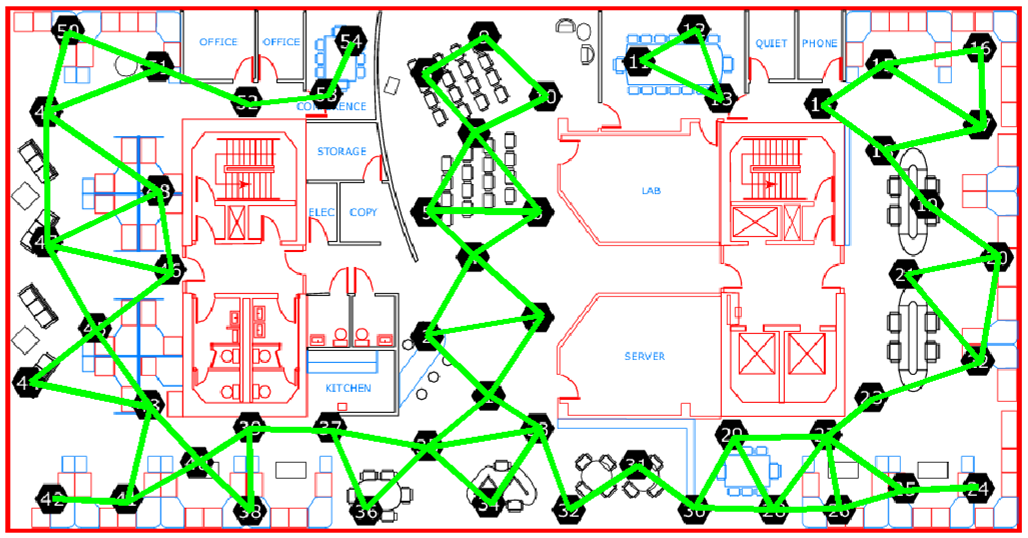
\includegraphics[width=0.5\textwidth]{expected.png}
	\caption{Exptected Correlation}
\end{figure}

Thus, We can add spatial regularization for all neighboring sensor node pairs on our TR-MF model. 

\begin{equation*}\begin{aligned}
\frac{1}{2}\sum_{m,n}{(r_{m,n} - \hat{r}_{m,n})}^2 &+ \frac{\beta_1}{2}\sum_m{\mu_m^2} + \frac{\beta_2}{2}\sum_n{\mu_n^2}\\
&+ \frac{\beta_3}{2}\sum_m{||\mathbf{p}_m||^2} + \frac{\beta_4}{2}\sum_n{||\mathbf{q}_n||^2}\\ 
&+ \frac{1}{2}\gamma_1\sum{(\mu_m-\mu_{m+1})^2}\\ 
&+ \frac{1}{2}\gamma_2\sum{||\mathbf{p}_m-\mathbf{p}_{m+1}||^2}\\
&+ \frac{1}{2}\gamma_3\sum{(\mu_{n_i}-\mu_{n_j})^2} \\
&+ \frac{1}{2}\gamma_4\sum{||\mathbf{p}_{n_i}-\mathbf{p}_{n_j}||^2}.\\
\end{aligned}\end{equation*}


Table \ref{table:spatial_random_hum}, \ref{table:spatial_random_light}, \ref{table:spatial_random_tem}, \ref{table:spatial_temporal_hum}, \ref{table:spatial_temporal_light}, \ref{table:spatial_temporal_tem}  show the result of adding spatial regularization. STR-MF mean TR-MF with strong spatial regularization, while sTR-MF is with weak spatial regularization.

\begin{table} [htbp]
\setlength{\tabcolsep}{2pt}
\centering
\caption{RMSE of (berkeley, random, humidity)}
\label{table:spatial_random_hum}
\begin{tabular} {r | r r r}
	train	& TR-MF	&	STR-MF	&	sTR-MF	\\ \hline
	10\% & $ \mathbf{ 0.142 } $ & $ 0.484 $ & $ 0.173 $ \\
	20\% & $ \mathbf{ 0.114 } $ & $ 0.424 $ & $ 0.135 $ \\
	40\% & $ \mathbf{ 0.092 } $ & $ 0.352 $ & $ 0.104 $ \\
	60\% & $ \mathbf{ 0.082 } $ & $ 0.337 $ & $ 0.093 $ \\
	80\% & $ \mathbf{ 0.076 } $ & $ 0.324 $ & $ 0.084 $ \\
	85\% & $ \mathbf{ 0.075 } $ & $ 0.326 $ & $ 0.083 $ \\
\end{tabular}
\end{table}


\begin{table} [htbp]
\setlength{\tabcolsep}{2pt}
\centering
\caption{RMSE of (berkeley, random, light)}
\label{table:spatial_random_light}
\begin{tabular} {r | r r r}
	train	& TR-MF	&	STR-MF	&	sTR-MF	\\ \hline
	10\% & $ \mathbf{ 35.480 } $ & $ 97.365 $ & $ 38.308 $ \\
	20\% & $ \mathbf{ 28.200 } $ & $ 90.645 $ & $ 28.869 $ \\
	40\% & $ \mathbf{ 21.190 } $ & $ 85.758 $ & $ 22.762 $ \\
	60\% & $ \mathbf{ 17.180 } $ & $ 83.251 $ & $ 18.334 $ \\
	80\% & $ \mathbf{ 17.740 } $ & $ 84.413 $ & $ 18.095 $ \\
	85\% & $ \mathbf{ 14.440 } $ & $ 81.972 $ & $ 15.828 $ \\
\end{tabular}
\end{table}


\begin{table} [htbp]
\setlength{\tabcolsep}{2pt}
\centering
\caption{RMSE of (berkeley, random, temperature)}
\label{table:spatial_random_tem}
\begin{tabular} {r | r r r}
	train	& TR-MF	&	STR-MF	&	sTR-MF	\\ \hline
	10\% & $ \mathbf{ 0.046 } $ & $ 0.154 $ & $ 0.061 $ \\
	20\% & $ \mathbf{ 0.032 } $ & $ 0.146 $ & $ 0.047 $ \\
	40\% & $ \mathbf{ 0.023 } $ & $ 0.145 $ & $ 0.037 $ \\
	60\% & $ \mathbf{ 0.018 } $ & $ 0.147 $ & $ 0.031 $ \\
	80\% & $ \mathbf{ 0.015 } $ & $ 0.148 $ & $ 0.027 $ \\
	85\% & $ \mathbf{ 0.016 } $ & $ 0.138 $ & $ 0.028 $ \\
\end{tabular}
\end{table}




\begin{table} [htbp]
\setlength{\tabcolsep}{2pt}
\centering
\caption{RMSE of (berkeley, temporal, humidity)}
\label{table:spatial_temporal_hum}
\begin{tabular} {r | r r r}
	train	& TR-MF	&	STR-MF	&	sTR-MF	\\ \hline
	10\% & $ 0.957 $ & $ 0.573 $ & $ \mathbf{ 0.547 } $ \\
	20\% & $ 0.796 $ & $ 0.657 $ & $ \mathbf{ 0.459 } $ \\
	40\% & $ 0.771 $ & $ 0.520 $ & $ \mathbf{ 0.455 } $ \\
	60\% & $ 0.540 $ & $ \mathbf{ 0.351 } $ & $ 0.708 $ \\
	80\% & $ 0.447 $ & $ 0.299 $ & $ \mathbf{ 0.261 } $ \\
	85\% & $ 0.323 $ & $ \mathbf{ 0.166 } $ & $ 0.256 $ \\
\end{tabular}
\end{table}

\begin{table} [htbp]
\setlength{\tabcolsep}{2pt}
\centering
\caption{RMSE of (berkeley, temporal, light)}
\label{table:spatial_temporal_light}
\begin{tabular} {r | r r r}
	train	& TR-MF	&	STR-MF	&	sTR-MF	\\ \hline
	10\% & $ \mathbf{ 220.070 } $ & $ 281.607 $ & $ 264.763 $ \\
	20\% & $ \mathbf{ 113.310 } $ & $ 236.865 $ & $ 230.054 $ \\
	40\% & $ \mathbf{ 58.090 } $ & $ 110.758 $ & $ 64.388 $ \\
	60\% & $ \mathbf{ 41.730 } $ & $ 150.149 $ & $ 69.235 $ \\
	80\% & $ \mathbf{ 21.450 } $ & $ 112.694 $ & $ 28.017 $ \\
	85\% & $ \mathbf{ 8.310 } $ & $ 85.423 $ & $ 12.079 $ \\
\end{tabular}
\end{table}


\begin{table} [htbp]
\setlength{\tabcolsep}{2pt}
\centering
\caption{RMSE of (berkeley, temporal, temperature)}
\label{table:spatial_temporal_tem}
\begin{tabular} {r | r r r}
	train	& TR-MF	&	STR-MF	&	sTR-MF	\\ \hline
	10\% & $ 0.515 $ & $ \mathbf{ 0.242 } $ & $ 0.307 $ \\
	20\% & $ 0.392 $ & $ \mathbf{ 0.179 } $ & $ 0.187 $ \\
	40\% & $ 0.310 $ & $ 0.196 $ & $ \mathbf{ 0.189 } $ \\
	60\% & $ 0.206 $ & $ \mathbf{ 0.191 } $ & $ 0.243 $ \\
	80\% & $ 0.132 $ & $ \mathbf{ 0.108 } $ & $ 0.114 $ \\
	85\% & $ 0.088 $ & $ \mathbf{ 0.065 } $ & $ 0.082 $ \\
\end{tabular}
\end{table}

